\title{INF564 Project report}
\documentclass[paper=a4, fontsize=11pt]{scrartcl}
\usepackage[utf8]{inputenc}
\usepackage[T1]{fontenc}
\usepackage{fourier}

\usepackage[francais]{babel}
\usepackage[protrusion=true,expansion=true]{microtype}	
\usepackage{amsmath,amsfonts,amsthm}
\usepackage{hyperref}
\usepackage{minted}
\usepackage{graphicx}

\usepackage{sectsty}
\allsectionsfont{\centering \normalfont\scshape}

\usepackage[nottoc, notlof, notlot]{tocbibind}

\usepackage{fancyhdr}
\pagestyle{fancyplain}
\fancyhead{}											% No page header
\fancyfoot[L]{}											% Empty 
\fancyfoot[C]{}											% Empty
\fancyfoot[R]{\thepage}									% Pagenumbering
\renewcommand{\headrulewidth}{0pt}			% Remove header underlines
\renewcommand{\footrulewidth}{0pt}				% Remove footer underlines
\setlength{\headheight}{13.6pt}

\numberwithin{figure}{section}			% Figurenumbering: section.fig#
\numberwithin{table}{section}				% Tablenumbering: section.tab#

\newcommand{\horrule}[1]{\rule{\linewidth}{#1}} 	% Horizontal rule

\title{	
		\usefont{OT1}{bch}{b}{n}
		\normalfont \normalsize \textsc{INF564 : Compilation} \\ [25pt]
		\horrule{0.5pt} \\[0.4cm]
		\huge Compilateur pour Mini-C en OCaml \\
		\horrule{2pt} \\[0.5cm]
}
\author{
		\normalfont 								\normalsize
        Lo\"{i}c Gelle\\[-3pt]		\normalsize
        19 mars 2017
}
\date{}


%%% Begin document
\begin{document}
\maketitle
\section{Introduction}

Ce court rapport a pour objet de présenter le travail effectué lors du projet du cours INF564 -- Compilation. La première partie explique la structure du projet et les choix techniques retenus. La deuxième partie explique le choix des environnements de développement et de tests ainsi que ses motivations. Enfin, la dernière partie évoque le débogage des tests finaux du projet.\\

Le code source du projet est disponible sur Github\footnote{Voir \url{https://github.com/loicgelle/inf564-compiler}}.

\section{Structure du projet et choix techniques}

La structure du projet suit assez simplement les étapes qui permettent de transformer le code source du programme d'entrée en code assembleur pour la machine cible.

\subsection{Front-end du compilateur : parseur et lexeur}

Les fichiers \texttt{code/lexer.mll} est utilisé par \textit{Menhir} pour le lexing, tandis que le parsing est réalisé avec \textit{ocamlyacc} et le fichier \texttt{code/parser.mly}. La commande \texttt{ocamlbuild} du \texttt{Makefile} permet de réaliser la compilation de ces fichiers de manière transparente.\\

En cas d'erreur lors du lexing, une exception est levée -- qui contient le message d'erreur le plus explicite possible ainsi que la position des lexèmes impliqués dans le code source -- et rattrapée par le point d'entrée du compilateur. Le parsing se charge de renvoyer un arbre syntaxique dont la syntaxe est décrite dans l'interface \texttt{ast.mli}.

\subsection{Analyse statique de typage}

Un typage de l'arbre syntaxique est réalisé dans le module \texttt{typer.ml}. Ce dernier renvoie un arbre syntaxique contenant des informations de typage et décrit par l'interface \texttt{ast\_typed.mli}. En cas d'erreur lors du typage, une exception est également levée et rattrapée par le point d'entrée du programme.\\

Afin d'éviter des copies en profondeur inutiles des environnements -- lors du typage des fonctions récursives, par exemple --, des structures de données non mutables sont utilisées pour représenter les environnements de typage :

\begin{minted}{ocaml}
module VarState = Map.Make(String)

type env_decl =
  | Env_var of typ
  | Env_struct of (env_decl VarState.t)
  | Env_fun of typ * typ list

let env = ref VarState.empty
\end{minted}

\subsection{Back-end du compilateur}

Les différentes passes de transformations réalisées sur l'arbre syntaxique typé sont effectuées par les modules \texttt{pass1\_to\_rtl.ml}, \texttt{pass2\_to\_ertl.ml}, \texttt{pass3\_to\_ltl.ml} et\newline \texttt{pass4\_to\_assembly.ml}. On notera que ces passes s'appuient sur des modules fournis dans le répertoire \texttt{code/mini-c}, et que les modules réalisant la construction du graphe d'interférence et l'analyse de durée de vie lors de la troisième passe sont placés dans le dossier \texttt{code/pass3\_utils}.\\

Comme pour l'analyse de typage, il arrive que l'on veuille modifier un environnement temporairement, le temps d'analyser un bloc. Dans le module \texttt{pass1\_to\_rtl.ml}, les environnements sont cette fois-ci représentés par des structures mutables -- des tables de hachage. Lorsqu'il est nécessaire de modifier temporairement un environnement, les modifications apportées sont stockées dans une variable dont on se sert par la suite pour restaurer l'environnement à son état initial. De cette manière, on ne réalise pas non plus de copie en profondeur des environnements, mais on utilise cette fois-ci une approche différente.

\subsection{Synthèse des différentes transformations}

Toutes les transformations effectuées sont lancées par le module \texttt{main.ml}, qui est le point d'entrée du programme et qui peut au besoin rattraper les exceptions levées lors de la compilation ou afficher des informations de débogage. Si on simplifie et qu'on oublie ces interactions avec le point d'entrée du programme, les étapes de transformation du code sont représentées en figure \ref{transformations}.

\begin{figure}[!ht]
    \center
    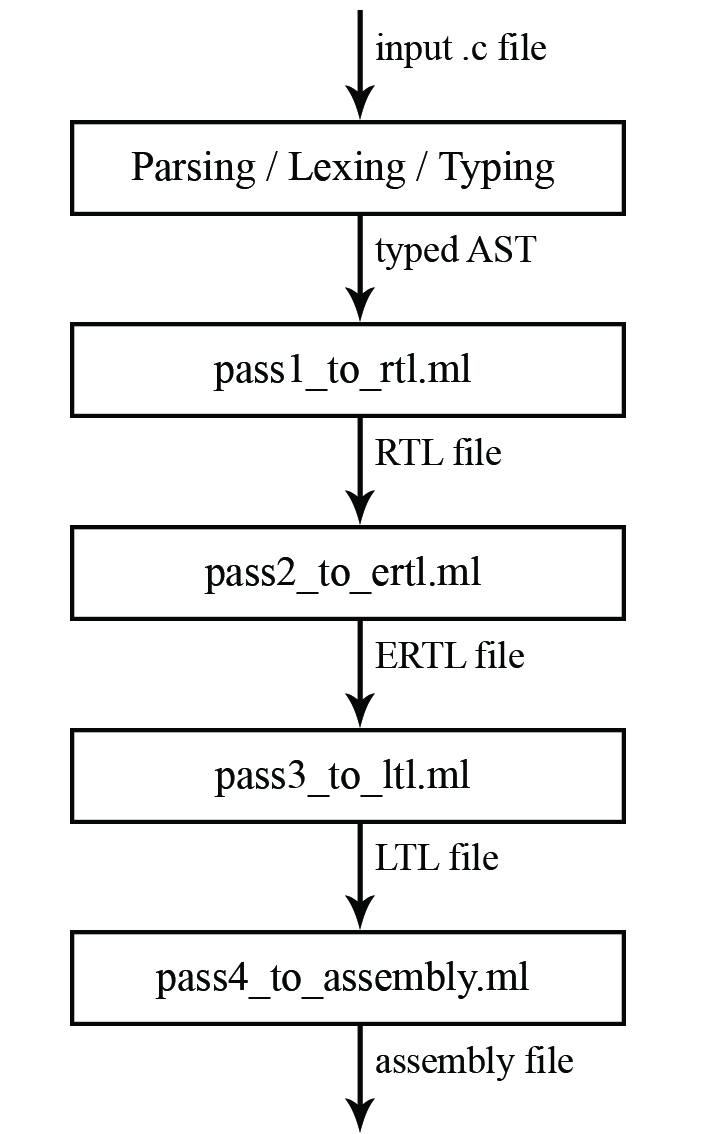
\includegraphics[width=0.3\textwidth]{./images/transformation_flow.jpg}
    \caption{\label{transformations} Les étapes de transformation du code.}
\end{figure}

\section{Environnements de développement et de test}

Le développement d'un logiciel, et plus particulièrement d'un compilateur, nécessite d'avoir un environnement de développement et un environnement de test cohérents entre eux. Il faut au moins que les deux environnements supportent le même assembleur et l'exécutent de la même manière.\\

Dans mon cas, ma plateforme de développement a une configuration avec Mac OS X alors que l'assembleur cible du projet est l'assembleur x86-64 Linux, qui est un peu différent. Le défi était alors de pouvoir tester le compilateur pendant le développement et de proposer un environnement de test autonome pour l'évaluation du projet. La solution la plus évidente est d'utiliser une machine virtuelle et d'y installer une distribution Linux pour le développement et les tests. Cependant, la virtualisation matérielle est gourmande en ressources et rend donc les développements laborieux, et le partage d'une machine virtuelle complète est lourd.\\

La solution que j'ai retenue a été d'utiliiser Docker\footnote{Voir ici : \url{https://www.docker.com/}}, une plateforme de containerisation. L'utilisation de containers présente les mêmes avantages que la virtualisation matérielle en termes d'isolation de l'application exécutée, mais elle est moins gourmande en ressources puisque l'application utilise directement le noyau du système d'exploitation hôte. Surtout, les containers Docker sont très simples de mise en place et d'utilisation. Dans le cadre du projet, la première étape est de construire un container de base qui contient toutes les dépendances du projet grâce à la commande \texttt{make docker-init} qui construit un container en puisant ses instructions dans le fichier \texttt{code/docker-base/Dockerfile} :

\begin{minted}{docker}
FROM ubuntu:latest

RUN apt-get update && \
    apt-get install -y build-essential gcc ocaml opam m4 && \
    opam init && \
    opam config env && \
    opam install ocamlbuild menhir
\end{minted}

Le container ainsi créé utilise donc un système Ubuntu minimal et y ajoute les dépendances nécessaires -- \texttt{gcc}, \texttt{ocaml}, \texttt{opam}, \texttt{ocamlbuild} et \texttt{menhir}. Une fois ce container créé, il sert de base au container final qui doit être reconstruit à chaque changement du code source. Le fichier utilisé pour ce dernier container est \texttt{code/Dockerfile} :

\begin{minted}{docker}
FROM compiler-base

COPY ./ /compiler/
WORKDIR /compiler
ENV PATH="/root/.opam/system/bin:${PATH}"

CMD echo $PATH && \
    ls /root/.opam/system/bin && \
    make && \
    make tests3
\end{minted}

On repart du container de base créé précédemment et on y copie le répertoire de développement du compilateur. Lorsqu'on lance ce container -- avec \texttt{make docker-tests} --, il exécute les instructions qui suivent la commande \texttt{CMD}, c'est-à-dire qu'il compile le projet et qu'il lance les tests. On obtient donc un environnement de test autonome à peu de frais.

\section{Tests finaux}

La plus grosse partie du débogage a eu lieu lors de la dernière passe de transformation du code vers le code assembleur cible. Parmi les difficultés rencontrées, on peut notamment évoquer :

\begin{itemize}
\item La gestion de la division : l'opérateur de division de l'assembleur présente quelques spécificités qu'il est difficile d'anticiper dès les premières étapes du développement. Il m'a fallu revenir dans les étapes précédentes pour vérifier l'ordre des opérandes, et ajouter des instructions pour gérer le cas des variables signées\footnote{Voir par exemple ici : \url{http://stackoverflow.com/questions/10343155/x86-assembly-handling-the-idiv-instruction}} ;
\item La gestion des tests unaires et binaires : les tests finaux ont été l'occasion de prendre du recul sur les transformations précédentes réservées aux structures conditionnelles, et d'effectuer quelques optimisations et modifications ;
\item La gestion des variables locales : les tests d'exécution utilisent parfois une variable locale qui a le même nom qu'une variable qui a une portée plus globale. En pratique, les étapes précédentes de la compilation géraient mal ce cas et il a fallu les modifier en conséquence ;
\item La gestion des étiquettes : lorsqu'on supprime une instruction de type \texttt{goto}, il faut faire attention à modifier en conséquence les instructions qui pointaient vers l'étiquette supprimée.
\end{itemize}

Je pense avoir réussi à effectuer un débogage méthodique et efficace en essayant d'abord de compiler correctement les programmes et les structures les plus simples. Je me suis pour cela aidé de fichiers d'exemple que j'ai créés pour les tests et qui m'ont permis de vérifier la bonne prise en charge de certaines structures du langage.

\end{document}